% !TeX spellcheck = en_US
\documentclass[]{ccs-thesis}
% options:
% [germanthesis] - Thesis is written in German
% [plainunnumbered] - Don't print numbers on plain pages
% [earlydraft] - Settings for quick draft printouts
% [watermark] - Print current time/date at bottom of each page
% [phdthesis] - switch to PhD thesis style
% [twoside] - double sided
% [cutmargins] - text body fills complete page


% Author name. Separate multiple authors with commas.
\author{Philip Frerk}
\birthday{March 31, 1994}
\birthplace{Bielefeld}

% Title of your thesis.
\title{Wireless Protection of Vulnerable Road Users}

% Choose one of the following lines. Feel free to change the word "Informatik" to match your degree program.
%\thesistype{Masterarbeit im Fach Informatik}\thesiscite{Master's Thesis~(Masterarbeit)}
%\thesistype{Bachelorarbeit im Fach Informatik}\thesiscite{Bachelor Thesis~(Bachelorarbeit)}
\thesistype{Seminar Thesis in Master's Computer Science}\thesiscite{Seminar Thesis~(Seminararbeit)}

% List of advisors, separated by commas.
\advisors{Christoph Sommer}

% List of referees, separated by commas.
\referees{Christoph Sommer, Falko Dressler}


% Define abbreviations used in the thesis here.
\acrodef{WSN}{Wireless Sensor Network}
\acrodef{MANET}{Mobile Ad Hoc Network}
\acrodef{ROI}{Region of Interest}{short-indefinite={an}, long-plural-form={Regions of Interest}}
\acrodef{ADAC}{German Automobile Association}{foreign={Allgemeiner Deutscher Automobilclub}}
\acrodef{CANhashing}[CAN]{Content Addressable Network}{extra={when referring to the distributed hash table}}
\acrodef{CANproto}[CAN]{Controller Area Network}{extra={when referring to the bus protocol}}
\acrodef{VU}{Vulnerable Road User}
\acrodef{V2PC}{Vehicle to Pedestrian Communication System}

\begin{document}

\pagenumbering{roman}

\maketitle

\chapter*{Abstract}
\addcontentsline{toc}{chapter}{Abstract}
\begin{otherlanguage*}{american}

about 1/2 page:
\begin{enumerate}
	\item Motivation (Why do we care?)
	\item Problem statement (What problem are we trying to solve?)
	\item Approach (How did we go about it)
	\item Results (What's the answer?)
	\item Conclusion (What are the implications of the answer?)
\end{enumerate}

Protecting vulnerable road users is a very important task as in roughly 50 \% of all traffic accidents vulnerable road users are involved. Vulnerable road users are pedestrians or drivers of two-wheeled vehicles.

A technology is needed that warns both the vulnerable road user and the car driver if an accident between them is likely to happen.  This is not an easy challenge because the warnings have to be sent in time  and also it has to ensured that no people are warned who are not really affected by the approaching car.

To achieve that goal, wireless networks, GPS and sensor perception will be used.

Results show that the number of accidents with vulnerable road users involved can be reduced dramatically.

Therefore, much more work will be put into this topic, because it is already shown that the technologies can potentially prevent many traffic accidents.

\end{otherlanguage*}


\chapter*{Kurzfassung}
\addcontentsline{toc}{chapter}{Kurzfassung}
\begin{otherlanguage*}{ngerman}

Gleicher Text (sinngemäß, nicht wörtlich) in Deutsch

\end{otherlanguage*}
\acresetall

\cleardoublepage
\tableofcontents
\TODO{The table of contents should fit on one page. When in doubt, adjust the \texttt{tocdepth} counter.}

\cleardoublepage
\pagenumbering{arabic}


\chapter{Introduction}
\label{chap:introduction}

\TODO{umstrukturieren, vielleicht doch keine sektionen!}

\section{Motivation}
\label{sec:motivation}

Within the last century the usage of motorized vehicles has grown rapidly. While this fact brings the great benefit of full mobility, it does not come without its downsides. One of them is the high number of traffic accidents. According to~\cite{v2pcomm} in roughly half of all traffic accidents, \acp{VU} are involved. Hence, there is huge potential to prevent injuries or even deaths of many people. This thesis will give you an overview of the current state of research in this area. While there are many approaches beyond the discipline of Wireless Networking (e.g. Computer Vision for pedestrian recognition), this thesis will focus mainly on how to prevent traffic accidents by using wireless network technology. However, the other areas will also be explained briefly since they often work hand in hand with Wireless Networking.

\section{Structure of the Thesis}
\label{sec:structure}

The thesis is structured as follows. First, in chapter~\ref{chap:v2p} we will look at so called \acp{V2PC} which use wireless networks in order for pedestrian and vehicles to communicate so that accidents between them can be prevented.

Second, in chapter~\ref{chap:perception} we will look at detecting \acp{VU} by using perception of cars. We will only shortly dive into this topic, because it is not directly connected to Wireless Networking. Nevertheless, it is necessary to know the basics in order to understand chapter~\ref{chap:fusion}.

There, a combination of \acp{V2PC} and perception will be used to improve the protection of \acp{VU}.

Finally, in chapter~\ref{chap:conclusion} all the approaches will be summarized and also we will see what future tasks are still left in this area to make it usable in the real world.


\chapter{V2P Communication Systems}
\label{chap:v2p}

\begin{enumerate}
\item erst das standard zeug 
\item dann das mit beacon weil es besser ist
\item am ende noch erwähnen dass es trotzdem noch nicht reicht wegen unpräzisem GPS
\end{enumerate}

The basic idea behind \acp{V2PC} is that a driving vehicle (most often a car) and a \ac{VU} (most often a pedestrian) exchange messages over a wireless network in order tell each other their positions. By doing that, accidents between them can be prevented because both the car driver and the pedestrian can react to the received messages.

There are several approaches to implements such a system and they will be discovered in this chapter.

\section{With special Device}\label{sec:special device}

First, we will look at such communication systems which use a special device for the \ac{VU} in order to send his messages. In \cite{v2pprotection} and \cite{watchover} such systems have been proposed. 

The device from \cite{v2pprotection} can be seen in the bottom of figure~\ref{fig:device}. In the top of figure~\ref{fig:device} you can see the warning unit that will be installed in the car.

\begin{figure}[h]
	\centering
	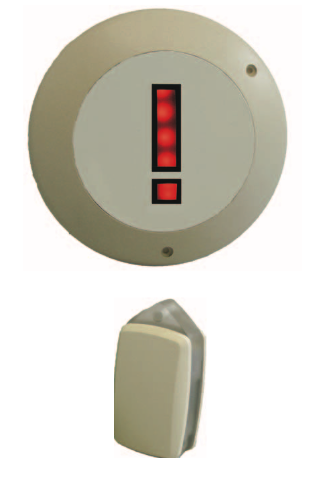
\includegraphics[width=0.3\textwidth]{figures/1_device}
	\caption{The Warning Unit for Cars and the Warning Device for Pedestrians from \cite{v2pprotection}}%
	\label{fig:device}%
\end{figure}

The task of the device for the pedestrian is to periodically send \enquote{Hello}-Messages including the pedestrian's position so that the warning unit in the car can receive those messages and detect a probably dangerous situation. Then the warning unit sets itself into a warning status (which can be seen in figure~\ref{fig:device}).

It is very important that the car driver does not get too many warning messages because otherwise he would loose sensibility for the warning. Therefore, a key issue is to ensure that only warning are created if the distance between car and pedestrian decreases gradually.

Figure~\ref{fig:chart1} shows the ratio of meaningful warnings divided by the number of all warning which is roughly 50\% because in this test scenario only one pedestrian is present. That ratio is not satisfying, but is only because of the low number of pedestrians.

In figure~\ref{fig:chart2} you see the same statistics, but for a scenario with 10 pedestrians. Here the same ratio is almost 100\%.

\TODO{hier fehlt noch warum die ratios so sind}

\begin{figure}[h]
	\centering
	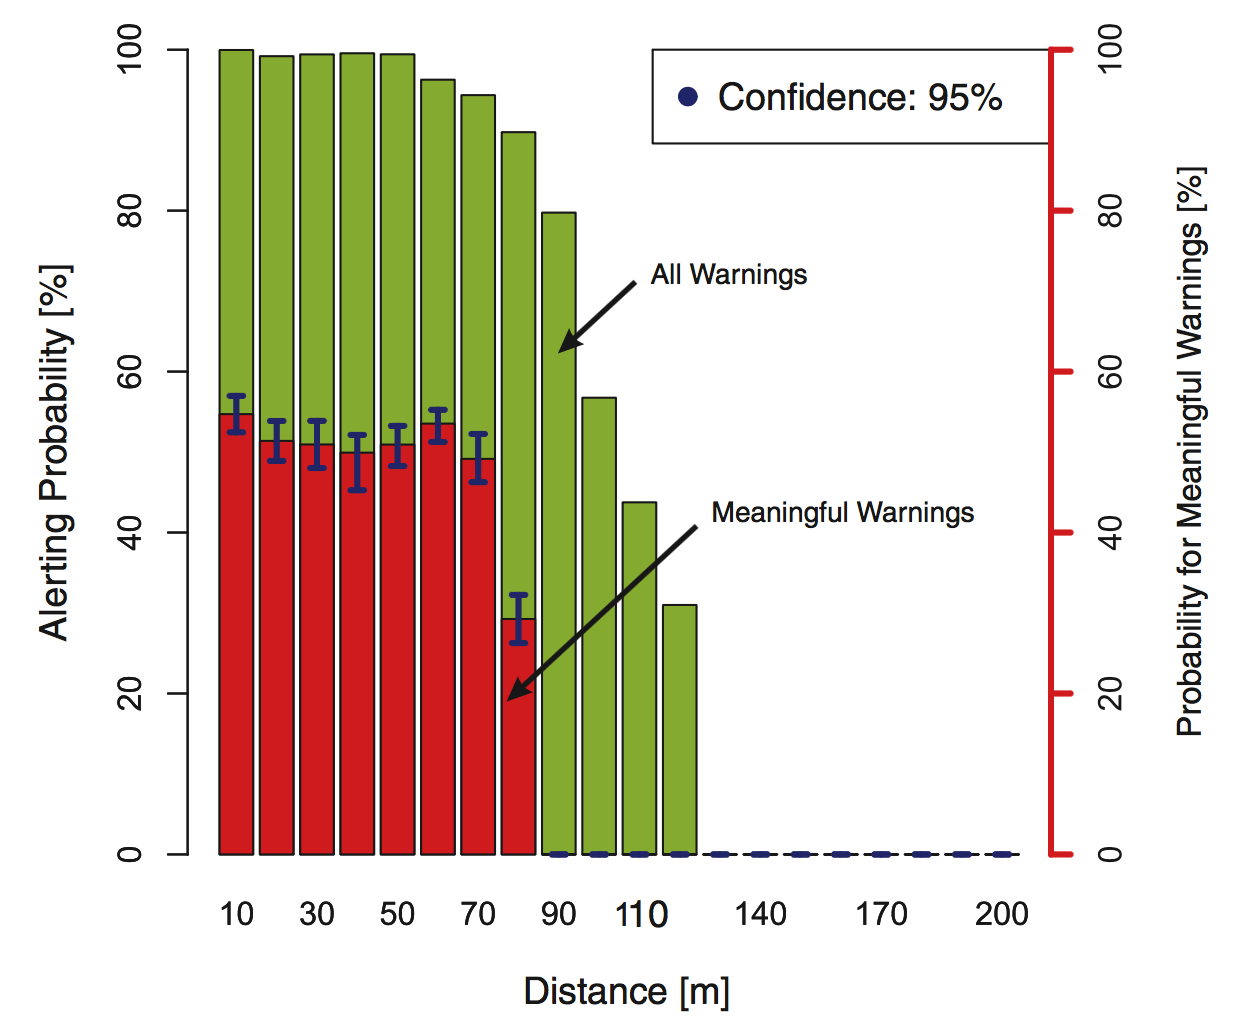
\includegraphics[width=0.8\textwidth]{figures/2_chart}
	\caption{Warning statistics in a test scenario with one pedestrian from \cite{v2pprotection}}%
	\label{fig:chart1}%
\end{figure}

\begin{figure}[h]
	\centering
	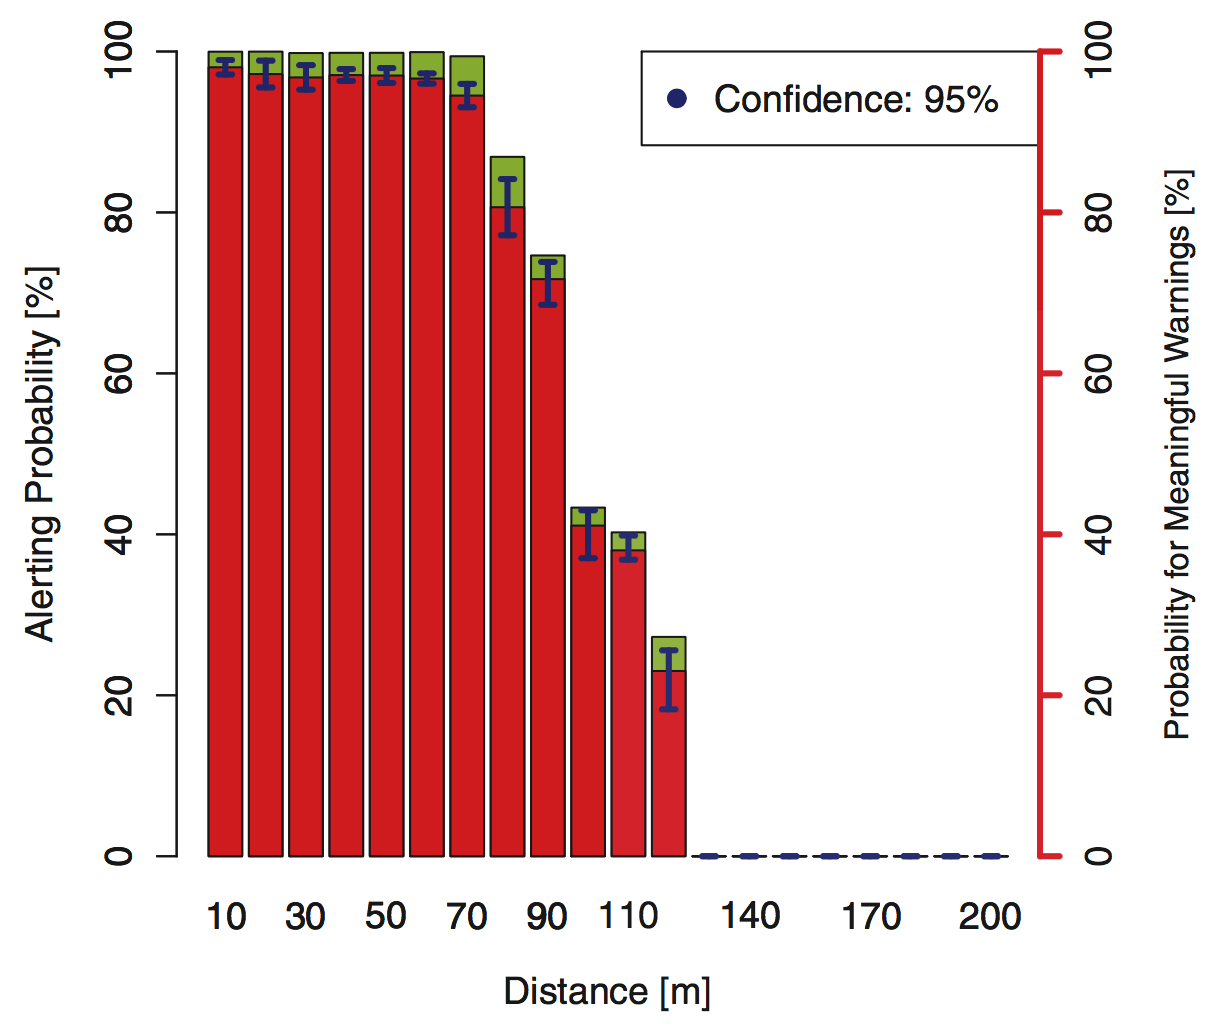
\includegraphics[width=0.8\textwidth]{figures/3_chart}
	\caption{Warning statistics in a test scenario with 10 pedestrians from \cite{v2pprotection}}%
	\label{fig:chart2}%
\end{figure}

\section{Using Smart Phones}

In \cite{v2pcomm}, another approach has been developed which has basically the same general idea as \cite{v2pprotection}, but is more detailed. Moreover, it has the great benefit that no additional device for the \ac{VU} is needed because in this system a smart phone or tablet will be used.

The approach is more detailed, because it formulates precise requirements that an implementation of a \ac{V2PC} should have in order to be able to work in reality. The  requirements are the following: One has to calculate a distance at which the warning messages are to be delivered. In section~\ref{sec:special device} we have already seen that this distance should not be too big, because otherwise too many meaningless warning would be received. But also, the distance must not be too small, because the pedestrian and the car driver must have enough time to react to the messages.



\chapter{Detecting Pedestrians by using Perception}
\label{chap:perception}

\TODO{Hier kommt nur ein kleiner Ausblick hin, da es nicht direkt etwas mit Wireless Networking zu tun hat}

\chapter{Fusion of Perception and V2P Communication}
\label{chap:fusion}




\chapter{Conclusion}
\label{chap:conclusion}


\begin{itemize}
\item summarize again what your paper did, but now emphasize more the results, and comparisons
\item write conclusions that can be drawn from the results found and the discussion presented in the paper
\item future work (be very brief, explain what, but not much how, do not speculate about results or impact)
\item recommended length: one page.
\end{itemize}



\cleardoublepage

\listofabbreviations
\clearpage

\listoffigures
\clearpage


\printbibliography

\end{document}
